\documentclass[10pt,landscape,a4paper]{article}
\usepackage{multicol}
\usepackage[landscape]{geometry}
\usepackage{hyperref}
\usepackage[utf8]{inputenc}
\usepackage{minted}
\usepackage{venndiagram}
\usepackage{graphicx}
\usepackage{cancel}
\usepackage{wasysym}
\usepackage{amssymb}
\usepackage{stmaryrd}
\usepackage{ulem}
\usepackage{color}
\usepackage{ifsym}


\geometry{top=1cm,left=1.5cm,right=1cm,bottom=1cm}

% Turn off header and footer
\pagestyle{empty}
 
% Redefine section commands to use less space
\makeatletter
\renewcommand{\section}{\@startsection{section}{1}{0mm}%
                                {-1ex plus -.5ex minus -.2ex}%
                                {0.5ex plus .2ex}%x
                                {\normalfont\large\bfseries}}
\renewcommand{\subsection}{\@startsection{subsection}{2}{0mm}%
                                {-1explus -.5ex minus -.2ex}%
                                {0.5ex plus .2ex}%
                                {\normalfont\small\bfseries}}
\renewcommand{\subsubsection}{\@startsection{subsubsection}{3}{0mm}%
                                {-1ex plus -.5ex minus -.2ex}%
                                {1ex plus .2ex}%
                                {\normalfont\footnotesize\bfseries}}
\renewcommand{\@venn@radius}{4mm}
\renewcommand{\@venn@overlap}{2mm}
\renewcommand{\@venn@vgap}{1mm}
\renewcommand{\@venn@hgap}{1mm}
\makeatother

% Don't print section numbers
\setcounter{secnumdepth}{0}

\setlength{\parindent}{0pt}
\setlength{\parskip}{0pt plus 0.5ex}

\newcommand{\sqljoin}[3]{
\begin{multicols*}{2}
  \begin{venndiagram2sets}
    #1
  \end{venndiagram2sets}
  \vfill\columnbreak
  \hspace{-8em}
  \begin{tabular}{ll}
    x & y \\
    \hline
    #2
  \end{tabular}
\end{multicols*}
\mint{sql}{#3}
}

\newcommand{\sql}[1]{\mintinline{sql}{#1}}



% -----------------------------------------------------------------------

\begin{document}

\footnotesize
\begin{multicols*}{3}


% multicol parameters
% These lengths are set only within the two main columns
%\setlength{\columnseprule}{0.25pt}
\setlength{\premulticols}{1pt}
\setlength{\postmulticols}{1pt}
\setlength{\multicolsep}{1pt}
\setlength{\columnsep}{2pt}

\section{Begriffe}

\begin{description}
\item[Datenbanksystem (DBS)]{Datenbankmanagementsystem DBMS + $n \cdot$ Datenbasen/Datenbestände/Datensätze\\(=strukturierte Sammlung von Daten)}
\item[Anforderungen an DBMS]{Redundanzfreiheit + Datenintegrität}
\item[Datenintegrität]{Datenkonsistenz(logische Widerspruchsfreiheit der Daten), Datensicherheit(Schutz vor physischem Verlust) \& Datenschutz(Zugriffe)}
%\textcolor{red}{\item[Data Dictionary/Datenkatalog]{enthält alle Meta-Daten/Systemdaten, Daten welche die Struktur der Anwendungsdaten beschreiben}}
\item[Datenmodelle]{Hierarchisch, Netzwerk, Relationen, Postrelational: Objektrelational (Methoden, Tabellenvererbung,
    \sout{1. NF}), Objektorientiert (analog Programmiersprache)}
\item[DBMS-Funktionen]Transaktionen, Mehrbenutzerbetrieb, Sicherheit, Backup \& Recovery, Datenkatalog, SQL
\end{description}
\section{Architektur}

\begin{description}
\item[Tier]{\textit{1-Tier}: DBMS im selben Prozess wie Client (MS Access),\\ 
\textit{2-Tier}:
    Client, Server mind. prozessmässig getrennt}

\item[3-Ebenen Modell]\textit{externe Ebene}: Sicht auf Teilmenge der DB, Applikationen, externes Schema
\textit{konzeptionelle/logische Ebene}: konzeptionelles Schema/Modell/Entwurf(UML), logisches Modell/Datenbankschema
\textit{interne Ebene}: physische Datenstruktur, internes Schema (DDL)
\end{description}
\section{UML}
Aggregation: $\lozenge$ Komposition: $\blacklozenge $\\
\textit{Abstrakte Klassen}\\
\underline{Objektname : Klassenname}\\
$[visibility] AttrName [multiplicity][:type] [=initial-value]$\\
$Name [0..1] : String$, $Salaer: float = 1000.0$

\subsection{Generalisierung/Spezialisierung}
\textbf{disjunkt: }1 Objekt$\rightarrow$Instanz \underline{einer} Unterklasse \{disjoint\}\\
\textbf{überlappend: }1 Objekt$\rightarrow$\underline{mehreren} Unterklassen \{overlapping\}\\
\textbf{vollständig: }Subklassen spezifiziert, keine zusätzlichen \{complete\}\\
\textbf{unvollständig: }nicht alle, zusätzliche erlaubt \{incomplete\}

%\subsection{Vermeidung Überlappung, Delegation}
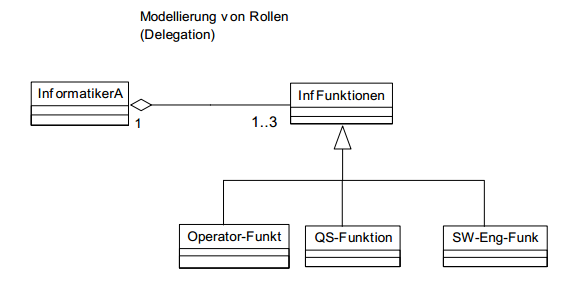
\includegraphics[scale=.5]{delegation.PNG}\\
\textbf{Entitätstyp: }Klasse \textbf{Entitätsmenge: }Alle Objekte einer Klasse, Relation \textbf{Krähenfüsschen: }c=optional, n/m=mehrere

\section{Relationales Modell}
\begin{description}
\item[Entitätsintegrität]Kein Primärschlüsselattribut \mintinline{SQL}{NULL}
\item[Referentielle Integrität]Fremdschlüsselattribute $\neq$ \mintinline{SQL}{NULL}, wenn Primärschlüssel existiert
\end{description}
  Student (
\underline{id} INTEGER, 
lang TEXT(3) NOT NULL UNIQUE, 
\textit{abt} INTEGER NOT NULL REFERENCES TableB(tableB\_id))  
\begin{description}
\item[Redundanzen] Mutationsanomalien: Einfüge-, Änderungs- & Löschanomalie
\item[Normalformen] 1. NF: Wertebereiche der Attribute atomar, 2. NF: Jedes Attr. \underline{voll} funktional abhängig von \underline{jedem} Schlüsselattr., 3. NF: Kein Nichtschlüsselattr. von irgendeinem Schlüssel transitiv abhängig, BCNF: Schlüsselkand. \{Name, Sportart\}\{Name, Verein\}, Verein $\rightarrow$ Sportart nicht erlaubt!!!
\item[Regeln]optionale Assoziationen (0..*)$\rightarrow$wenige?$\rightarrow$Zwischentabelle, Assoziative Klassen: Zwischentabelle + die beiden fk = pk
\end{description}

\section{SQL Data Definition Language}
\mintinline{SQL}{CREATE DATABASE foo WITH OWNER = 'bar';}\\
\sql{CREATE INDEX indexname ON tbl_name (attr.);}
\begin{minted}{SQL}
CREATE TABLE Angestellter (
PersNr   INTEGER NOT NULL, --Column Constraint
Name     VARCHAR(20) NOT NULL,
Tel      TEXT NULL,
Salaer   FLOAT NOT NULL,
EintrittsDatum DATE DEFAULT CURRENT_DATE,
--Table Constraints 
PRIMARY KEY (PersNr, Name), 
CHECK (Salaer BETWEEN 1000 AND 20000)
);
\end{minted}
\begin{minted}{SQL}
ALTER TABLE team 
 ADD CONSTRAINT constraintbezeichnung 
	FOREIGN KEY (fk_stadion) REFERENCES 
	stadion (stadion_id); --Foreign Keys immer so
	

\end{minted}
\textbf{Referentielle Integrität} B abhängig von A\\
\mintinline{SQL}{ON [DELETE|UPDATE] CASCADE}\\
Tupel in B wird ebenfalls gelöscht/Referenz wird geändert\\
\mintinline{SQL}{ON [DELETE|UPDATE] RESTRICT}\\
Solange Referenz besteht, kann A nicht gelöscht werden (default)\\
Änderung wird nicht ausgeführt (default)\\
\mintinline{SQL}{ON [DELETE|UPDATE] SET NULL}\\
Fremdschlüsselattr. in Tupel B wird auf NULL gesetzt\\
\mintinline{SQL}{ON [DELETE|UPDATE] SET DEFAULT}\\
Fremdschlüsselattr. in Tupel B wird auf den Defaultwert gesetzt

\section{SQL Data Manipulation Language}
\mintinline{sql}{INSERT INTO Abteilung (Name, AbtNr) VALUES ('F&E', 20);}\\
\sql{INSERT INTO tbl_name (attr.) SELECT ...;}\\
\mintinline{sql}{UPDATE Abteilung SET abtnr=21 WHERE abtnr=20;}

\subsection{Queries}
\mintinline{sql}{SELECT DISTINCT...} Duplikate werden unterdrückt\\
\begin{description}
\item[Projektion]{$\pi_{\mathrm{foo, bar}}\mathrm{(tbl\_name)}$ \\
    \sql{SELECT foo, bar FROM A;}}\\
    Identische Tupel werden eliminiert
\item[Selektion]{$\sigma_{\mathrm{ID < 10}}(tbl\_name)$ \\
    \sql{SELECT * FROM A WHERE ID < 10;}}
\item[Kartesisches Produkt, CROSS JOIN]$R_1 \times R_2$\\
\sql{SELECT * FROM R1, R2; SELECT * FROM R1 CROSS JOIN R2;}
\item[Vereinigung]{$A \cup B$ \\
    \sql{SELECT * FROM A UNION [ALL] SELECT * FROM b;}}\\
    \mintinline{sql}{UNION ALL}$\rightarrow$Duplikate werden \underline{nicht} entfernt\\
    Schemata müssen gleich sein!
\item[Differenz, Komplement]$A - B$\\
\sql{SELECT * FROM A [EXCEPT] SELECT * FROM B}\\
Schemata müssen gleich sein!
\item[Umbenennung]{$\rho_{\mathrm{bar} \leftarrow \mathrm{foo}}\mathrm{(tbl\_name)}$ \\
  \sql{SELECT foo AS bar FROM ...;}}
\item[Durchschnitt]{$A \cap B$ \\
    \sql{SELECT * FROM A INTERSECT SELECT * FROM B;}}\\
    Schemata müssen gleich sein!
\end{description}

\subsection{Unterabfragen}
\mintinline{sql}{...WHERE Wohnort [NOT] IN ('Luzern', 'Zug', 'Horw')...}\\
\sql{...WHERE [NOT] EXISTS(SELECT * ...)}\\
\sql{WHERE attr. [<|>|...] [ANY|ALL] (SELECT * ...)}\\
Vergleiche mit \sql{NULL} (x $>$ \sql{NULL}) immer UNKNOWN\\
\sql{SELECT * FROM (SELECT * FROM ...) AS ["]alias["];}

\subsection{Aggregationsfunktionen}
\mintinline{SQL}{MAX, MIN, AVG, SUM, COUNT}\\
\sql{NULL}-Werte werden ignoriert (Ausnahme: \sql{COUNT})\\
\mintinline{SQL}{SELECT [Aggrfkt.](attr.) FROM tabl GROUP BY group, subgroup}\\
\mintinline{sql}{GROUP BY...HAVING [Aggrfkt.](...)...;}\\
$\rightarrow$analog \mintinline{sql}{WHERE}, aber für Aggregationsfunktionen

\subsection{Window functions}
\sql{SELECT [Aggrfkt.](attr) OVER (PARTITION BY ... ORDER BY...)}\\
Mit \sql{PARTITION BY} wird gruppiert\\
\sql{lag|lead (attr., offset, default) OVER (ORDER BY...)}\\
vorderer/hinterer Wert innerhalb der Partition wird ausgegeben\\
Defaultmässig offset=1, default=\sql{NULL}

\subsection{Common Table Expression (CTE)}
\sql{WITH tmp AS (SELECT...) SELECT * FROM tmp;}\\
Rekursiv:
\begin{minted}{sql}
WITH RECURSIVE cte (spalten) AS
   (Ursprungsselect UNION ALL Rekursionsselect)
SELECT spalten FROM cte WHERE ...;
\end{minted}

Beispiel:

\begin{minted}{sql}
WITH RECURSIVE unter ( persnr, name, chef ) AS
   (SELECT A.persnr, A.name, A.chef FROM angestellter A
    WHERE A.chef = 1010    UNION ALL
    SELECT A.persnr, A.name, A.chef FROM angestellter A
    INNER JOIN unter B on B.persnr = A.chef
) SELECT * FROM unter ORDER BY chef, persnr;
\end{minted}

\subsection{Views}
\begin{minted}{sql}
CREATE VIEW AngPublic (Persnr, Name, Tel, Wohnort) AS
SELECT Persnr, Name, Tel, Wohnort
FROM Angestellter;
\end{minted}
Bedingungen für updatable: nur 1 \sql{FROM}-Eintrag, kein \sql{WITH,}\sql{DISTINCT},\sql{GROUP BY,}\sql{HAVING,} \sql{LIMIT,}\sql{OFFSET,}\sql{UNION,}\sql{INTERSECT,} \sql{EXCEPT}, keine Aggregationen, window function 

\subsection{Joins}
\textbf{Theta-Join} $\sigma_{=, >,<, <=, >=, <>}(R_1 \times R_2)=\bowtie_{=, >, ...}$\\
\textbf{Equi-Join} $\sigma_{a.x = b.y}(A \times B)$\\
\textbf{\mintinline{SQL}{NATURAL JOIN}} Automatisch alle gleichnamigen Spalten verglichen und gejoint\\
\textbf{Linker Semi-Join $\ltimes$} $\pi_{\mathrm{Schema linker Relation}}\mathrm{(\mintinline{SQL}{NATURAL JOIN})}$\\
\textbf{Inner Join}\\
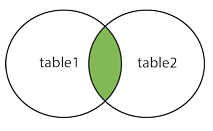
\includegraphics[scale=.1]{innerjoin.PNG}
\sql{SELECT * FROM a [INNER] JOIN b ON a.x = b.y;}\\
\mintinline{sql}{INNER muss nicht zwingend geschrieben werden}\\
\textbf{Left (Outer) Join} {\tiny \textifsym{d|><|}}\\
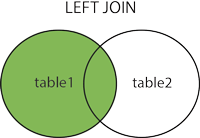
\includegraphics[scale=.1]{img_leftjoin.png}
\mintinline{SQL}{SELECT * FROM a LEFT [OUTER] JOIN b ON a.x = b.x;}\\
\mintinline{SQL}{OUTER} muss nicht zwingend geschrieben werden\\
right $\rightarrow$ dito\\
\textbf{Full (Outer) Join} {\tiny \textifsym{d|><|d}}\\
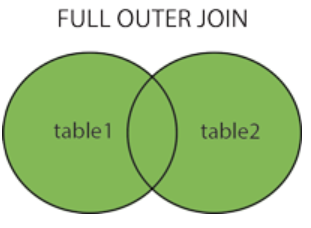
\includegraphics[scale=.1]{fullouterjoin.PNG}
\mintinline{SQL}{SELECT * FROM a [FULL] OUTER JOIN b ON a.x = b.x;}\\
\mintinline{SQL}{FULL} muss nicht zwingend geschrieben werden\\ \\
\mintinline{sql}{...JOIN LATERAL..}damit kann tabellenübergreifend auf Attr. zugegriffen werden
\subsection{Löschen}\\
\mintinline{sql}{DROP TABLE Angestellter CASCADE;}\\
Löscht zusätzlich alle Views + FK-Constraints\\
\begin{minted}
ALTER TABLE tbl_name
 DROP CONSTRAINT constraintbezeichnung;
\end{minted}
\mintinline{sql}{TRUNC[ATE] TABLE tbl_name}\\
Löscht nur der Inhalt der Tabelle\\
\mintinline{sql}{DELETE FROM Abteilung WHERE abtnr=21;}\\
Einzelne Tupel löschen

\subsection{Varia}
\sql{COALESCE(NULL, NULL, 'Hallo')}\\
erster Nullwert zurück$\rightarrow$Hallo wird zurückgegeben\\ 
\sql{ROUND(Zahl, Anz. Stellen)}\\
Ohne Angabe der Anz. Stellen$\rightarrow$keine Nachkommast.\\
\sql{CREATE TEMPORARY TABLE mytable (...)}$\rightarrow$besteht bis Ende der Transaktion/Session\\
\mintinline{sql}{ORDER BY [attrn., Spaltennr.] [ASC|DESC];}\\
Default: ASC (aufsteigend, kleinster Wert zuerst)\\
\mintinline{sql}{LIKE 'Zu\%'} \% = 0 bis * Zeichen\\
\mintinline{sql}{LIKE '____'} \_ entspricht genau 1 bel. Zeichen 

\section{SQL Data Control Language}
\begin{minted}{sql}
CREATE ROLE user/group WITH  LOGIN PASSWORD 'password'
[CREATEDB NOCREATEROLE];
\end{minted}\\
\sql{ALTER USER name WITH [CREATEDB ...]}\\
\sql{DROP ROLE name;}
\begin{minted}{sql}
GRANT [SELECT|INSERT|UPDATE|...] ON tbl_name
TO role [WITH GRANT OPTION]
\end{minted}
\sql{[WITH GRANT OPTION]}$\rightarrow$Rechte können weitergegeben werden\\
\sql{REVOKE [Recht] ON tbl_name FROM rolename}

\section{Transaktionen}
\textbf{A}tomicity (Vollständig/gar nicht), \textbf{c}onsistency (konsistentem Zustand$\rightarrow$n. konst. Zustand, \textbf{I}solation(Trans. von anderen isoliert), \textbf{D}urability (persistente Änderungen)

\subsection{SQL Transaction Control Language}
\sql{BEGIN TRANSACTION;} 
\sql{SET TRANSACTION ISOLATION LEVEL [...]}
\sql{COMMIT TRANSACTION;}
\sql{ROLLBACK TRANSACTION;}
\sql{SAVEPOINT name;}
\sql{RELEASE SAVEPOINT name;}
\sql{ROLLBACK TO SAVEPOINT name;}
\subsection{Konfliktpaare}
Zwei Transaktionen A,B | zwei Variablen\\
(r_A(x), r_B(y))$\rightarrow$kein Konflikt\\
Alle anderen, wenn x == y$\rightarrow$Konflikt!
\subsection{Pessimistisches Verfahren/Sperrprotokolle}
Exclusive Lock(x): RW, Shared Lock(s): R (mehrere gleichzeitig möglich)\\
\textbf{2 Phase Locking: }Growing: Sperren, Shrinking Phase: Sobald Transaktion ein Lock freigegeben hat$\rightarrow$keine weiteren Bezüge, Am Schluss Freigabe aller Locks, -Cascading Rollback -Deadlocks\\
\textbf{Strict 2PL: }Alle gehaltenen Sperren nach Ende der Transaktion freigegeben +kein Cascading Rollback
\subsection{Isolationlevels}
(-): unmöglich mit cursor stability\\
\begin{tabular}{lllll1}
  Level & Dirty & Fuzzy/Nonrep. & Lost upd. & Phantom \\
  \hline
  uncommitted & - & - & (-) & - \\
  \textbf{committed} & \checked & - & (-) & - \\
  Repeatable & \checked & \checked & \checked  & - \\
  Serializable & \checked & \checked & \checked & \checked
\end{tabular}\\

\textbf{Dirty Read}: liest uncommited data von anderer Transaktion
\textbf{Fuzzy/Nonrepeatable Read}: liest bereits gelesene Daten nochmals gleich ein, Daten wurden jedoch geändert 
\textbf{Lost Update}: Zwei Transaktionen verändern Info, erste durch zweite überschrieben
\textbf{Phantom Read}: Liest gleiche Daten mehrmals, neue oder gelöschte Werte\\
\textbf{committed}: Sicht eines Snapshots vor Query (nur committed data ersichtlich), Änderungen innerhalb Transaktion ersichtlich
\textbf{Repeatable}: Sicht eines Snapshots vor Transaktion,  Änderungen innerhalb Transaktion ersichtlich

\subsubsection{Snapshot Isolation (SI)} 
Änderungen$\rightarrow$Objekte = Snap?Nein$\rightarrow$Rollback\\
Keine Cascading Rollbacks, Deadlocks möglich

\subsection{Multi-Version Concurrency Control (MVCC)}
Schreiben: erzeugt neue Version, lesen: immer von aktuellster, Schreiber blockieren andere Schreiber

\section{Index}
Grad = k, k = $\frac{m}{2}$ = Min. Anzahl an Einträgen, \\
m = 2k = Max. Anzahl an Einträgen, max 2k+1 Unterknoten\\
17 in B-Baum einfügen:\\
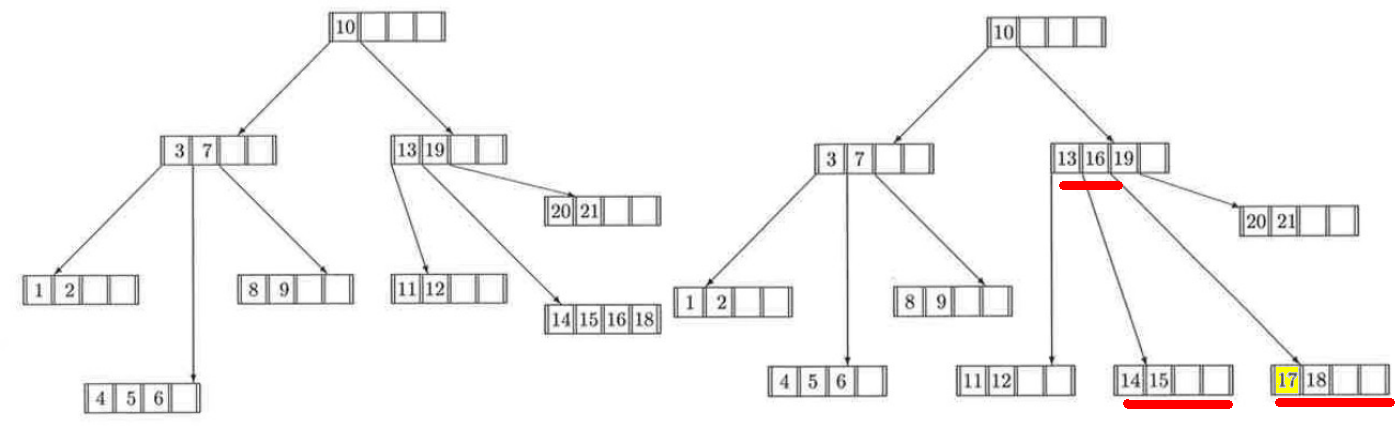
\includegraphics[width=\columnwidth]{bbaum.png}

\textbf{Indexalg: }ISAM, B-Bäume, B+-Bäume, Hash, BRIN, Bitmap(Bitmuster) 
\textbf{Indexvarianten}(\textit{\sout{in Postgres}}): Clustered Index, Primär Index, \textit{Sekundär-Index}, zusammengesetzter Index, \textit{partieller Index}, funktionaler Index,
mehrstufige, mehrdimensionale

\section{JDBC}
\subsection{Treibertypen}
1. JDBC-ODBC-Brücke, 2. Native plattformeigene JDBC-Treiber, 3. Universeller JDBC-Treiber (Java), 4. Direkte Netzwerktreiber (Java)

\begin{minted}{Java}
try (Connection connection = DriverManager.getConnection
 ("jdbc:postgresql:mydb", username, password)) {

try (Statement statement = connection.createStatement()) {
 ResultSet resultSet = statement.executeQuery
 ("SELECT * FROM Account");
 while (resultSet.next()) {/*Start: vor erster Zeile*/
 String owner = resultSet.getString("Owner");/*oder über Index*/
 int balance = resultSet.getInt("Balance");/*NULL wird zu 0*/
 }}
} catch (SQLException e) {
}/*Keine Verbindung, Login fehlgeschlagen*/
\end{minted}

\begin{minted}{Java}
PreparedStatement statement = connection.prepareStatement(
"UPDATE Account SET Balance = Balance + ? WHERE Owner = ?");
statement.setInt(1, -100);
statement.setString(2, "Bob");
statement.execute();
\end{minted}

\textbf{SQL-Injection}\sql{-'; UPDATE coffees SET price=price/2; --}

\subsection{Transaktionen}
\begin{minted}{SQL}
connection.setAutoCommit(false);
connection.setTransactionIsolation(TRANSACTION_SERIALIZABLE)
/*Impliziter Transaktionsbeginn (erstes Statement)*/
connection.commit();
connection.rollback();/*Für Exception-Handling*/
\end{minted}

\subsection{MetaData}
\sql{connection.getMetaData()}: SQL-Sprachumf., DB-Produktname, Driver-Eig., Datentypen, Eigenschaften Transaktionen, ...
\sql{resultSet.getMetaData()}$\rightarrow$ResultSetMetaData

\subsection{Scrollable/Updateable ResultSet}
\sql{createStatement()}-Parameter: \sql{TYPE_FORWARD_ONLY}: kann nicht scrollen \sql{TYPE_SCROLL_INSENSITIVE},\sql{TYPE_SCROLL_SENSITIVE}: reflektiert [keine] Änderung von anderen, \sql{CONCUR_READ_ONLY}, \sql{CONCUR_UPDATABLE}\\

\sql{rs.moveToInsertRow(); rs.updateString("Owner"); rs.insertRow();}

\subsection{Batch Updates}
Default: jedes Statement = 1 Roundtrip, Batch Updates sammelt
\begin{minted}{sql}
statement.addBatch("INSERT|UPDATE|DELETE");
statement.addBatch("CREATE|DROP|ALTER");
int [] rowUpdateCount = statement.executeBatch();
\end{minted}

\end{multicols*}
\end{document}                                                                                                                                                                                                                                                                                                                                                                                                                                                                                                                                                                                                                                                                                                                                                                                                                                                                                                                                                                                                                                                                                                                                                                                                                                                                                                                                                                                                                                                                                                                                                                                                                                                                                                                                                                                                                                                                                                                                